%% 
%% Copyright 2007-2020 Elsevier Ltd
%% 
%% This file is part of the 'Elsarticle Bundle'.
%% ---------------------------------------------
%% 
%% It may be distributed under the conditions of the LaTeX Project Public
%% License, either version 1.2 of this license or (at your option) any
%% later version.  The latest version of this license is in
%%    http://www.latex-project.org/lppl.txt
%% and version 1.2 or later is part of all distributions of LaTeX
%% version 1999/12/01 or later.
%% 
%% The list of all files belonging to the 'Elsarticle Bundle' is
%% given in the file `manifest.txt'.
%% 
%% Template article for Elsevier's document class `elsarticle'
%% with harvard style bibliographic references

\documentclass[preprint,12pt,authoryear]{elsarticle}

%% Use the option review to obtain double line spacing
%% \documentclass[authoryear,preprint,review,12pt]{elsarticle}

%% Use the options 1p,twocolumn; 3p; 3p,twocolumn; 5p; or 5p,twocolumn
%% for a journal layout:
%% \documentclass[final,1p,times,authoryear]{elsarticle}
%% \documentclass[final,1p,times,twocolumn,authoryear]{elsarticle}
%% \documentclass[final,3p,times,authoryear]{elsarticle}
%% \documentclass[final,3p,times,twocolumn,authoryear]{elsarticle}
%% \documentclass[final,5p,times,authoryear]{elsarticle}
%% \documentclass[final,5p,times,twocolumn,authoryear]{elsarticle}

%% For including figures, graphicx.sty has been loaded in
%% elsarticle.cls. If you prefer to use the old commands
%% please give \usepackage{epsfig}

%% The amssymb package provides various useful mathematical symbols
\usepackage{amssymb}
%% The amsthm package provides extended theorem environments
%% \usepackage{amsthm}

%% The lineno packages adds line numbers. Start line numbering with
%% \begin{linenumbers}, end it with \end{linenumbers}. Or switch it on
%% for the whole article with \linenumbers.
%% \usepackage{lineno}
\usepackage{xcolor}
\usepackage{rotating}

\journal{The Lancet}

\begin{document}

\begin{frontmatter}

%% Title, authors and addresses

%% use the tnoteref command within \title for footnotes;
%% use the tnotetext command for theassociated footnote;
%% use the fnref command within \author or \affiliation for footnotes;
%% use the fntext command for theassociated footnote;
%% use the corref command within \author for corresponding author footnotes;
%% use the cortext command for theassociated footnote;
%% use the ead command for the email address,
%% and the form \ead[url] for the home page:
%% \title{Title\tnoteref{label1}}
%% \tnotetext[label1]{}
%% \author{Name\corref{cor1}\fnref{label2}}
%% \ead{email address}
%% \ead[url]{home page}
%% \fntext[label2]{}
%% \cortext[cor1]{}
%% \affiliation{organization={},
%%            addressline={}, 
%%            city={},
%%            postcode={}, 
%%            state={},
%%            country={}}
%% \fntext[label3]{}

\title{Protection provided by covid-19 vaccines and previous infection against the Omicron variant}

%% use optional labels to link authors explicitly to addresses:
%% \author[label1,label2]{}
%% \affiliation[label1]{organization={},
%%             addressline={},
%%             city={},
%%             postcode={},
%%             state={},
%%             country={}}
%%
%% \affiliation[label2]{organization={},
%%             addressline={},
%%             city={},
%%             postcode={},
%%             state={},
%%             country={}}

\author{}

\affiliation{organization={},%Department and Organization
            addressline={}, 
            city={},
            postcode={}, 
            state={},
            country={}}

\begin{abstract}
{\bf Background} The Omicron variant of the SARS-CoV-2 virus harbours a range of mutations, which confer to it a degree of immune evasion with respect to previous variants. We studied the extent of this evasion of post-vaccination and post-infection immunity in relation to time elapsed, using national health data from the Czech Republic.\\
{\bf Methods} Based on individual-level data on all laboratory-confirmed SARS-CoV-2 infections in the Czech Republic collected by the national Institute of Health Information and Statistics between December 7, 2021 and February 6, 2022, we used a Cox proportional hazards model and a logistic regression model to estimate the relative risk of reinfection, infection after vaccination, hospitalization (further subdivided into a need for oxygen therapy or intensive care) and death of Delta and Omicron variants, adjusting for sex, age, previous infection, vaccine type and vaccination status. \\
{\bf Findings} With the exception of Ad26.COV2-S vaccine (Johnson\&Johnson) we observed a time-dependent decline in vaccine effectiveness (VE) against Omicron with significantly lower VE compared to the Delta variant at all studied time points. A recently (within 61 days) completed two-dose vaccination without any previous infection reached a VE of 43\% (95\% CI: 42-44) against Omicron infection compared to 73\% (95\% CI: 72-75) against Delta. A recent mRNA booster dose increased VE to 55\% (95\% CI: 55-56) against Omicron infection compared to 90\% (95\% CI: 90-91) for Delta. The VE against Omicron hospitalization of a recent complete vaccination was 45\% (95\% CI: 30-58), and 87\% with a recent booster dose  (95\% CI: 84-89). The VE against the need for oxygen therapy was 57\% (95\% CI: 33-72) for recent complete vaccination, 90\% (95\% CI: 87-92) for a recent booster. The observed differences in VE between vaccines were small. \textcolor{red}{Post-infection immunity against the Omicron infection declined over time from HR 0.32 (95\% CI: 0.32-0.33) for a recent previous infection (60 days-6 months) to 0.84 (95\% CI: 0.82-0.86) for an infection 14+ months previously compared to na\"ive individuals. A recent combination of a previous infection and vaccination was more protective than either alone, with HR of Omicron infection below 0.2 and mostly below 0.15 for hospitalization regardless of the exact sequence of events.} Once infected, the odds ratio for Omicron relative to Delta is 0.36 (95\% CI: 0.34-0.38) for hospitalization, 0.24 (95\% CI: 0.22-0.26) for oxygen therapy, 0.24 (95\% CI: 0.21-0.28) for ICU admission and 0.14 (95\% CI: 0.09-0.22) for death.\\
{\bf Interpretation} The observed protection afforded by post-infection or post-vaccination immunity is lower for the Omicron than the Delta variant, supporting the existing data on its immune evasion. Both further decline over time. Especially recent booster vaccine doses or a combination of post-infection and post-vaccination immunity appear significantly protective  against both Omicron infection and the risk of a severe disease, suggesting a clear benefit of vaccines for already vaccinated and previously infected individuals, particularly if administered shortly before an epidemic wave. \\
{\bf Funding} No external funding was used to conduct this study.
\end{abstract}

%%Graphical abstract
%\begin{graphicalabstract}
%\includegraphics{grabs}
%\end{graphicalabstract}

%%Research highlights
%\begin{highlights}
%\item Research highlight 1
%\item Research highlight 2
%\end{highlights}

%\begin{keyword}
%% keywords here, in the form: keyword \sep keyword

%% PACS codes here, in the form: \PACS code \sep code

%% MSC codes here, in the form: \MSC code \sep code
%% or \MSC[2008] code \sep code (2000 is the default)

%\end{keyword}

\end{frontmatter}

%% \linenumbers

%\section*{Research in context}
%\noindent
%{\bf Evidence before this study} \\
%This section should include a description of all the evidence
%that the authors considered before undertaking this study.
%Authors should briefly state: the sources (databases, journal or
%book reference lists, etc) searched; the criteria used to include
%or exclude studies (including the exact start and end dates of
%the search), which should not be limited to English language
%publications; the search terms used; the quality (risk of bias)
%of that evidence; and the pooled estimate derived from meta
%analysis of the evidence, if appropriate.
%XXX \\[1ex]
%Accumulating evidence from several countries indicates that the effectiveness of covid-19 vaccines against infection declines in time, from about 80-90\% shortly after completing the vaccination to about 50-60\% and even less after 6 months. Published studies also suggest a significant boosting in vaccine effectiveness against infection about one week after the third vaccine dose. However, these observations come from different and often limited data sets. Moreover, the existing studies do not compare the decline in vaccine effectiveness with a decline in infection-based immunity in unvaccinated individuals. \\[1ex]
%{\bf Added value of this study} \\
%Authors should describe here how their findings add value to
%the existing evidence.
%In this study, we bring together data on infections caused by the Omicron variant of the SARS-CoV-2 virus, vaccinations (including booster doses), hospital admissions and deaths to estimate how the protection due to vaccination or previous SARS-CoV-2 infection declines with time, for the whole population of the Czech Republic. 
%Our findings show an overall decrease in vaccine effectiveness over time and a large increase after the administration of a booster dose. At the same time we show a fairly stable and high post-infection immunity over the study period. We hope this evidence will contribute to a better understanding of the changing impact of vaccines and previous infection in complex, real-world environments, which is crucial for the development of more effective and more easily communicated public health policies. \\[1ex]
%Our risk-based analyses indicate that while the vaccine effectiveness against infection, hospital admission or death declines in time at vaccine-specific rates. The observed decrease in vaccine effectiveness can be partly explained by an increased risk due to the delta variant. The administration of a booster dose returns the protection against infection back to about 95\%. The post-infection immunity decreases over time too, but at a lower rate: a protection of about 70\% is observed 18 months after infection. \\[1ex]
%{\bf Implications of all the available evidence} \\
%Authors should state the implications for practice or policy
%and future research of their study combined with existing
%evidence
%Our results strongly support a timely and widespread application of booster vaccine doses since their application appears to restore the vaccine-induced protection to the levels attained soon after completing the original vaccination scheme. 

%% main text
\section{Introduction}
\label{sec1}

The B.1.1.529 (Omicron) variant of SARS-CoV-2 was first detected in South Africa in November 2021, immediately designated a variant of concern by the WHO \citep{who2021omicron} and  thereafter seen quickly to spread throughout most of the world. This rapid spread was, at least in part, brought about by a degree of immune evasion due to a large number of mutations in the viral S-protein, which led to changes in epitopes recognised by antibodies elicited by vaccination or previous infection \citep{mccallum2022}. Together with non-pharmacological interventions such as face masks, distancing, ventilation of interior spaces, testing and isolating, vaccination ranks among the most effective means of individual and collective protection from the impacts of the pandemic. The immune evasion by the Omicron variant thus caused concern and led to a lot of interest in both laboratory and real-life epidemiological data that would accurately measure this phenomenon.

%Soon after evidence has accumulated indicating that the effectiveness of covid-19 vaccines declines in time to about 50-60\% and even less after six months (REFS), and that booster vaccine doses return the protection against the by then dominating Delta variant to or above the effectiveness values reached just after completing the original vaccination scheme (REFS), the world started to be invaded by a new variant of concern, the Omicron variant (REFS). Indeed, it is its high transmission abilities and risks of evading both vaccine-induced and post-infection immunity that forced the World Health Organization to declare this variant as a VOC on November 26, 2021 (REFS).

%The actual evidence from a number of counties, including Denmark, UK, France and the United States, confirms these concerns: the infection incidence increases at an unprecedented rate, jeopardizing functioning of many societal services (REFS). Unfortunately, these rates and the corresponding peaks of the `Omicron wave' are hard to predict by means of mathematical models, mainly since data on the vaccine and post-infection protection against Omicron are still rare and uncertain (REFS). 

Since December 27, 2020 the inhabitants of the Czech Republic have been receiving covid-19 vaccines, with the largest number vaccinated with the mRNA vaccine Comirnaty (BNT162b2, Pfizer/BioNTech), followed by Spikevax (mRNA-1273, Moderna), and the adenovirus-based vector vaccines Vaxzevria (ChAdOx1 nCoV-19, AstraZeneca) and Janssen Covid-19 Vaccine (Ad26.CoV2.S, Johnson\&Johnson, further abbreviated as Janssen). The overall population vaccination rate reached 70\% by XX.XX.2022 with significant differences among the various age groups (REF) %The rate of vaccination was increasing until the beginning of June, 2021, stayed relatively low during summer months, and started to rise again in October 2021, in response to epidemic control measures requiring a proof of infection/vaccination/negative test in many public places \citep{mzcr}. The administration of booster doses in the Czech Republic started on September 20, 2021 and was initially open to all individuals who completed their vaccination 8 months or longer ago with only Comirnaty and Spikevax as allowed boosting vaccines. The waiting period was shortened to 6 months on October 29, 2021. Until November 1, 2021 a full 100 \textmu g dose of Moderna was being administered as a booster dose and since that day only a 50 \textmu g dose was used.

The first case of the Omicron variant in the Czech Republic was detected at the end of November 2021. Whereas the proportion of the Omicron variant among new cases was estimated to be around 15\% on December XX, 2021 (REFS), by January 10, 2022 it became the dominant variant (REFS). An increasing number of infections among the fully vaccinated and re-infections indeed suggests that immune evasion poses a significant risk of further covid-19 development \citep{mzcr}. In this study, we estimate how the protection due to vaccination or previous SARS-CoV-2 infection against covid-19 infection and hospital admission develop in time, for the entire population of the Czech Republic.

\section{Methods}
\label{sec2}

\subsection{Study population and data sources}

The analyses are based on data from the Czech National Information System of Infectious Diseases (ISID), which includes records of all individuals tested positive for SARS-CoV-2 in the Czech Republic since the beginning of covid-19 pandemic, including children \citep{komenda2020}. This database is overseen by the Czech Ministry of Health and operated by the Institute of Health Information and Statistics of the Czech Republic. The ISID data is routinely collected in compliance with  Act No. 258/2000 Coll. on the Protection of Public Health. 
%Due to this legal mandate, our retrospective analyses required neither approval by an ethics committee nor informed consents from participants. 
The data collection was managed and its usage approved by the Institute of Health Information and Statistics of the Czech Republic, according to the rules set by the Ministry of Health of the Czech Republic. According to a decision of the Institute of Health Information and Statistics of the Czech Republic, our retrospective analyses did not require ethical approval.
Among other things, the ISID database covers demographic data (age, sex and region of residence), dates of vaccination, including the vaccine types for each dose, and dates of infection and potential reinfection, hospitalization including treatment, and the date of potentially  covid-19 related death. Some (approximately half in the studied period) records include information on whether it is the Omicron or other variant. Additional information on deaths from any cause come from the Death Certificate System; these data are used for censoring purposes only.

{\color{blue} TO APPENDIX: In total, our dataset contains 8,282,080 records of vaccinated and/or SARS-CoV-2 positive persons, out of which 10.937 were excluded for either inconsistency or the lack of valid gender and/or age information. An additional 97,855 records were excluded as corresponding individuals who died before 2021-12-7 which we set as the start date (34,145 were recorded as deceased from covid, 63,740 for other reasons) see Table \ref{description1}). 
As the source dataset consists only of those who  tested positive and/or were vaccinated, we expanded the sample to the whole population such that the added subjects  neither tested positive nor were vaccinated. In particular, we expanded each sex-age category to the numbers reported by the Czech Statistical Office by December 31, 2020 -- 10,701,777 inhabitants; consequently, our sample truly reflected the sex and age structure of the entire population, containing all the positive and/or vaccinated individuals. We neglected births and deaths of the added persons.} 

\subsection{Vaccine types and vaccination and infection dynamics}

In the Czech Republic, all EMA-approved Covid-19 vaccines have been distributed and used: the mRNA-based vaccines Comirnaty (BNT162b2, Pfizer/BioNTech) and Spikevax (mRNA-1273, Moderna), and the adenovirus-based vector vaccines Vaxzevria (ChAdOx1 nCoV-19, AstraZeneca) and Janssen Covid-19 vaccine (Ad26.CoV2.S, Johnson\&Johnson). 
%They were provided to all individuals at no cost following the Czech public health insurance system. Starting on December 27, 2020, workers in the critical infrastructure were vaccinated first, followed since January 15, 2021 by persons of age 80 and older (Table \ref{table:vaccination_schedule} in the Supplementary material). 
As of January XX, 2022, the Czech Institute of Health Information and Statistics reported 6,287,356 individuals completing the vaccination (58.75\% of the population and 67.36\% of persons age 12 years and older).%; see Fig.\,\ref{vaccrollout}.
Moreover,  1,996,080 individuals had been infected with SARS-CoV-2 virus as of January XX, 2022, out of which 12,894 (0.65\%) were reinfected.%; see Fig.\,\ref{fig:infection_dynamics}. 
See also Tables \ref{description1} and \ref{description2} for an overview of the numbers of infection-related outcomes and vaccines applied within various age cohorts.

%\begin{figure}[h]
%\centering\includegraphics[width=0.7\textwidth]{vaccination.png}
%\caption{Dynamics of vaccination in the Czech Republic. Specific days in which vaccination was open to an age group or professional or other category are specified in Table \ref{table:vaccination_schedule} in the Supplementary Material.}
%\label{vaccrollout}
%\end{figure}

%The covid-19 epidemic in the Czech Republic started with the first three cases reported on March 1, 2020 and was initially fueled by Czech citizens returning from the alpine ski resorts of Italy and Austria. Since then the country saw five waves of covid-19 spread. As of November 20, 2021, 1,996,080 individuals were infected with SARS-CoV-2 virus, of which 12,894 (0.65\%) were reinfected; see Fig.\,\ref{fig:infection_dynamics}. See also Tables \ref{description1} and \ref{description2} for an overview of the numbers of infection-related outcomes and vaccines applied within various age cohorts. 
%\subsection{Outcomes}

{\color{blue} To appendix: ?
We aggregate the time delays in two-month (61 days) periods with the last one lasting forever. In particular, we consider one such period after the first dose, four periods after the second one and two after the booster dose. When the new dose applies, (s)he is no longer regarded to be in any period corresponding to the previous dose, but enters the first period corresponding to the new dose. In line with the Czech vaccination recognition policy, the first period corresponding to any of the first two doses starts two weeks after the dose application, while for boosters this interval is just 7 days. For  reinfections, we consider nine two-month periods.

Since there are only several hundred booster doses of Vaxzevria and Janssen vaccines, we examine boosting effects only by the mRNA vaccines Comirnaty and Spikevax. Subjects with the alleged application of Vaxzevria (in total 176) or Janssen (in total 332) boosters are thus withdrawn from the study of booster dose effectiveness, as these records are most likely data entry errors. }

\subsection{Statistical analysis}

We separately studied four types of events: (i) SARS-CoV-2 infection defined as a PCR confirmed positive test of a person from any sample regardless of the presence of symptoms, (ii) hospital admission of a person tested positive with a PCR test, (iii) use of ventilator or other  oxygen therapy (kyslík, hfno, ventilátor, sry, nevím jak přeložit) and (iv) admission to ICU (all testing or treatment within two weeks before hospital admission and at any time during hospitalization),

We examined events during the two month period from 7/12/2021 to 13/2/2022, during which Delta and Omicron switched dominance in the Czech Republic. See TableOrGraph(data zde v Source Filed/variant.txt) for the overview of the infection numbers and the proportions of the particular variants as well as  infections of an undetermined origin. 
%Moreover, we estimated how HRs of infection after vaccination depended on time after the vaccine application (adjusted for sex, age and time since the last infection), how HRs of hospital admission or death depended on time after the vaccine application (adjusted for sex and age), and how HRs of reinfection in unvaccinated individiuals depended on time since the previous infection (adjusted for sex and age). In all these cases, we estimated the vaccine effectiveness ($\mbox{VE}$, regarding a previous infection as a ``vaccine'') as $\mbox{VE} = 1 - \mbox{HR}$ \citep{Chemaitelly2021, cohn2021, tartof2021effectiveness}. Subjects were withdrawn from the study at the time of their (covid or non-covid) death.


A Cox regression with time-varying covariates was applied to estimate hazard ratios (HRs) for the outcomes of interest separately for each variant -- in these analyses,  infections by the other variants or infections lacking discrimination were censored at the time of infection. Analogously to \cite{tartof2021effectiveness}, we used calendar time instead of time from event occurrence as the time scale. The time course of individual cases was thus modelled by means of ``switching'' dummy variables, corresponding to the stages of the process the subject goes through (by 61-dey periods for vaccination and 121-day periods for the time from the last infection).
The vaccine effectiveness is calculated by comparing hazards of the vaccinated and/or immunized individuals to those of the  ``control group'' -- those who have not been vaccinated or infected so far. In addition, we separately examine post-infection immunity by estimating hazard ratios for infection of previously unvaccinated individuals in dependence on  time from the infection. By using calendar time, we could automatically check the changing conditions of the epidemics, including adopted non-pharmaceutical measures, seasonal effects and the prevalence of the examined virus variant, as all these phenomena can then be encompassed in the baseline hazard function. 






To examine the probabilities of hospitalization, oxygen therapy and ICU admission given that the individual had been infected, we used logistic regression with the event of interest as outcome and with all discriminated infection types as the data. By means of the dummy corresponding to the virus variant, we can compare the probabilities of the outcome for both variants. Post-infection and -vaccination status, age and sex are used as control variables here. To estimate the effectiveness of vaccination and/or post-infection immunity, we run the logistic regression separately for the infections by individual variants (ale nevím, jestli to Luděk nakonec použije).

 
All calculations were performed using the R software (package \verb|survival|). The algorithm used to transform data from the database into the package command inputs was coded in C++. See Supplementary material for details. 

\section{Results}
\label{sec3}

\subsection*{Protection against infection}

As usual, we start with protection by vaccination and/or previous infection against infection, since this characteristic determines a potential for indirect protection of the non-infected and non-vaccinated persons. Regarding vaccination and the Omicron variant, protection reached 43\% (95\% CI 42-44) shortly after completing the full vaccination scheme, falling to 11\% (95\% CI 10-11) after two months. Protection jumped back to 55\% (95\% CI 55-56) after applying the booster dose, followed by a decline to 20\% (95\% CI 18-22) after two additional months. This strongly contrasts with protection against the Delta variant, where all these numbers are consistently higher, with respective protection levels of 73\% (95\% CI 72-75), 57\% (95\% CI 57-58), 90\% (95\% CI 90-91) and 81\% (95\% CI 79-84). Similar degrees of protection against infection are also provided by the post-infection immunity: 69\% (95\% CI 68-70) shortly after infection and 13\% (95\% CI 11-14) after four months for Omicron, versus 95\% (95\% CI 94-96) shortly after infection and 83\% (95\% CI 82-84) after four months for Delta. See also Figure \ref{figIalone} for a graphical comparison.

\begin{figure}[h]
\centering
%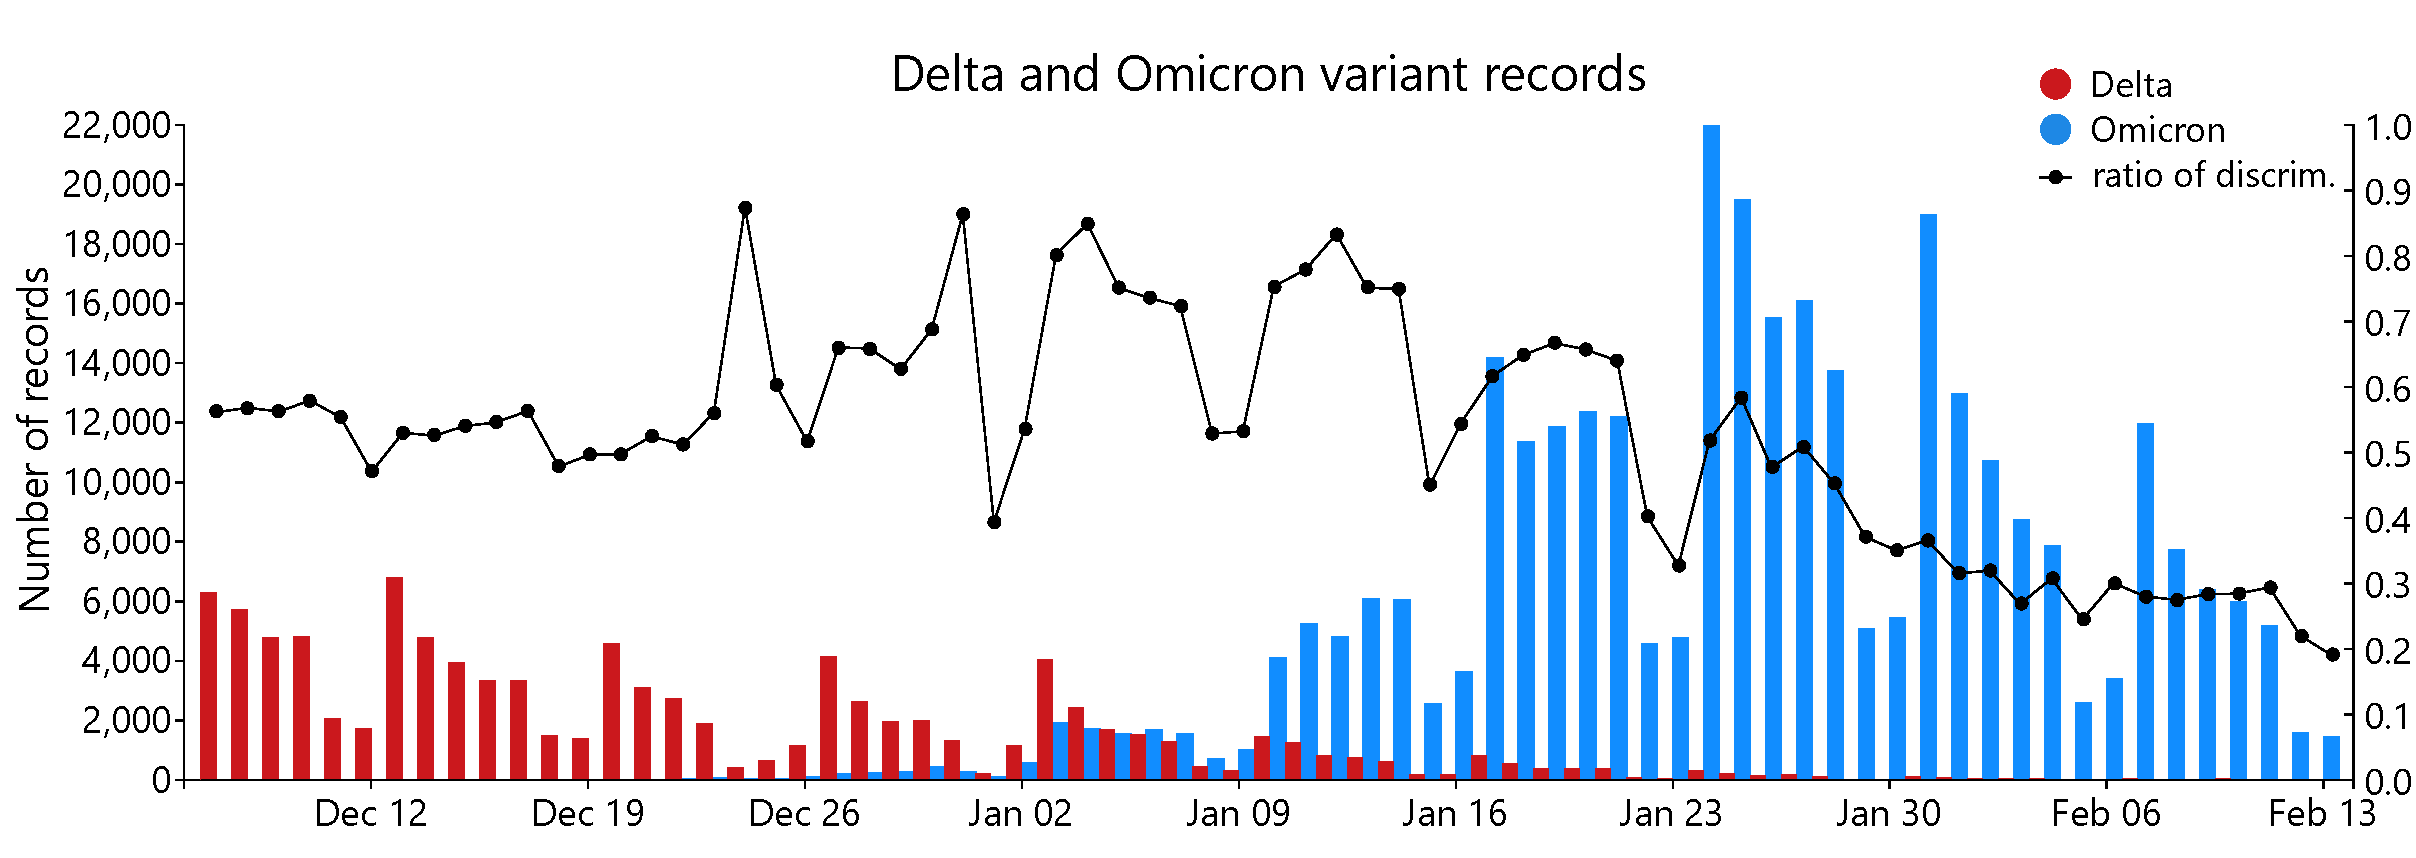
\includegraphics[width=0.9\textwidth]{fig1.pdf}
\caption{Protection by vaccination and/or previous infection against infection by the Omicron and Delta variants of the SARS-CoV-2 virus.}
\label{figIalone}
\end{figure}

We had enough data to examine all combinations in which previous infection preceded vaccination. As expected, VE declined with time elapsed from previous infection or vaccination (Tables \ref{tabIOinteractions} and \ref{tabIDinteractions}). For the Delta variant, any combination provided $>95\%$ protection against infection (Table \ref{tabIDinteractions}). This protection also remained quite high for Omicron when the previous infection was recent, falling to lower values for older infection, but even then VE was significantly higher than for vaccination or previous infection alone (Table \ref{tabIOinteractions}). The numbers below the respective Tables suggest that when protection is high (Delta) then the order of events does not matter. However, when protection is lower (Omicron), previous infection following vaccinations appears to provide higher VE than vice versa. 

\begin{table}[!h]
\caption{Protection due to various combinations of vaccination and past infection against infection, for the Omicron variant of the SARS-CoV-2 virus. In parentheses, 95\% credible intervals (CI) are given. \\[1ex]}
\label{tabIOinteractions}
\centering
\begin{tabular}{lcccc}
\hline
 & Booster 1 & Full 1 & Booster 2+ & Full 2+ \\
\hline
Infection 1 & 93\% (89-95) & 82\% (75-87) & 82\% (71-88) & 86\% (85-88) \\
Infection 2+ & 73\% (73-74) & 77\% (76-78) & 48\% (44-51) & 46\% (45-47) \\
\hline
\end{tabular} \\[1ex]
Further ... Boost2+/Inf1: 99\% (99-100), Full2+/Inf1: 90\% (88-91)
\end{table}

\begin{table}[!h]
\caption{Protection due to various combinations of vaccination and past infection against infection, for the Delta variant of the SARS-CoV-2 virus. In parentheses, 95\% credible intervals (CI) are given. \\[1ex]}
\label{tabIDinteractions}
\centering
\begin{tabular}{lcccc}
\hline
 & Booster 1 & Full 1 & Booster 2+ & Full 2+ \\
\hline
Infection 1 & 95\% (63-99) & 100\% (100-100) & 100\% (100-100) & 97\% (94-98) \\
Infection 2+ & 98\% (98-99) & 98\% (97-98) & 95\% (90-97) & 96\% (95-96) \\
\hline
\end{tabular} \\[1ex]
Further ... Boost2+/Inf1: 100\% (100-100), Full2+/Inf1: 96\% (90-98)
\end{table}

\subsection*{Protection against hospitalization}

Qualitatively analogous comparisons yet quantitatively consistently higher numbers arise as regards protection against hospitalization (Tables \ref{tabHalone}, \ref{tabHOinteractions} and \ref{tabHDinteractions}) and a need of oxygen therapy (Tables \ref{tabOalone}, \ref{tabOOinteractions} and \ref{tabODinteractions}). %, and hospitalization and a need of intensive care (Table \ref{tabUalone}). 
For example, recent booster dose provides 87\% protection against hospitalization and 90\% against a need of oxygen therapy of the Omicron variant. Moreover, apart from older infection and older vaccination, all combinations of previous infection and vaccinations that were present in data indicate $>90\%$ protection against Omicron, and most of them even $>95\%$. 

\begin{table}[!h]
\caption{Vaccine effectiveness and protection provided by post-infection immunity against hospitalization, for the Omicron and Delta variants of the SARS-CoV-2 virus. In parentheses, 95\% credible intervals (CI) are given. \\[1ex]}
\label{tabHalone}
\centering
\begin{tabular}{lcc}
\hline
Effect & Omicron & Delta \\
\hline
Full vaccination (first 2 months) & 45\% (30-58) & 73\% (66-78) \\
Full vaccination (after 2 months) & 32\% (24-39) & 78\% (76-79) \\
Booster dose (first 2 months) & 87\% (84-89) & 97\% (97-98) \\
Booster dose (after 2 months) & 79\% (75-82) & 96\% (94-97) \\
Infection (first 4 months) & 73\% (55-84) & 100\% (100-100) \\
Infection (after 4 months) & 66\% (54-75) & 94\% (91-96) \\
\hline
\end{tabular}
\end{table}

\begin{table}[!h]
\caption{Protection due to various combinations of vaccination and past infection against hospitalization, for the Omicron variant of the SARS-CoV-2 virus. In parentheses, 95\% credible intervals (CI) are given. \\[1ex]}
\label{tabHOinteractions}
\centering
\begin{tabular}{lcccc}
\hline
 & Booster 1 & Full 1 & Booster 2+ & Full 2+ \\
\hline
Infection 1 & $-$ & $-$ & $-$ & $-$ \\
Infection 2+ & 95\% (91-97) & 94\% (78-99) & 90\% (77-95) & 75\% (67-81) \\
\hline
\end{tabular} \\[1ex]
Further ... Boost2+/Inf1: 100\% (99-100), Full2+/Inf1: 94\% (79-99)
\end{table}

\begin{table}[!h]
\caption{Protection due to various combinations of vaccination and past infection against hospitalization, for the Delta variant of the SARS-CoV-2 virus. In parentheses, 95\% credible intervals (CI) are given. \\[1ex]}
\label{tabHDinteractions}
\centering
\begin{tabular}{lcccc}
\hline
 & Booster 1 & Full 1 & Booster 2+ & Full 2+ \\
\hline
Infection 1 & $-$ & $-$ & $-$ & $-$ \\
Infection 2+ & 99\% (98-100) & 97\% (91-99) & 98\% (85-100) & 98\% (98-99) \\
\hline
\end{tabular} \\[1ex]
Further ... Boost2+/Inf1: 100\% (100-100), Full2+/Inf1: 97\% (92-99)
\end{table}

\begin{table}[!h]
\caption{Vaccine effectiveness and protection provided by post-infection immunity against hospitalization and a need of oxygen therapy, for the Omicron and Delta variants of the SARS-CoV-2 virus. In parentheses, 95\% credible intervals (CI) are given. \\[1ex]}
\label{tabOalone}
\centering
\begin{tabular}{lcc}
\hline
Effect & Omicron & Delta \\
\hline
Full vaccination (first 2 months) & 57\% (33-72) & 81\% (75-86) \\
Full vaccination (after 2 months) & 37\% (25-47) & 81\% (79-82) \\
Booster dose (first 2 months) & 90\% (87-90) & 98\% (97-98) \\
Booster dose (after 2 months) & 85\% (80-88) & 97\% (95-98) \\
Infection (first 4 months) & 81\% (40-94) & 98\% (98-98) \\
Infection (after 4 months) & 88\% (72-94) & 96\% (94-98) \\
\hline
\end{tabular}
\end{table}

\begin{table}[!h]
\caption{Protection due to various combinations of vaccination and past infection  against hospitalization and a need of oxygen therapy, for the Omicron variant of the SARS-CoV-2 virus. In parentheses, 95\% credible intervals (CI) are given. \\[1ex]}
\label{tabOOinteractions}
\centering
\begin{tabular}{lcccc}
\hline
 & Booster 1 & Full 1 & Booster 2+ & Full 2+ \\
\hline
Infection 1 & $-$ & $-$ & $-$ & $-$ \\
Infection 2+ & 98\% (93-99) & 100\% (100-100) & 94\% (76-98) & 86\% (75-92) \\
\hline
\end{tabular} \\[1ex]
Further ... Boost2+/Inf1: 100\% (100-100), Full2+/Inf1: 100\% (100-100)
\end{table}

\begin{table}[!h]
\caption{Protection due to various combinations of vaccination and past infection  against hospitalization and a need of oxygen therapy, for the Delta variant of the SARS-CoV-2 virus. In parentheses, 95\% credible intervals (CI) are given. \\[1ex]}
\label{tabODinteractions}
\centering
\begin{tabular}{lcccc}
\hline
 & Booster 1 & Full 1 & Booster 2+ & Full 2+ \\
\hline
Infection 1 & $-$ & $-$ & $-$ & $-$ \\
Infection 2+ & 99\% (98-100) & 97\% (90-99) & 100\% (100-100) & 99\% (98-99) \\
\hline
\end{tabular} \\[1ex]
Further ... Boost2+/Inf1: 100\% (100-100), Full2+/Inf1: 100\% (100-100)
\end{table}

\subsection*{Logistic regressions}

Finally, our logistic regression analyses suggest that, once infected, the odds ratio  is 0.36 (0.34-0.38) for hospitalization with Omicron relative to Delta;  0.24 (0.22-0.26) for need of oxygen therapy with Omicron relative to Delta;  0.24 (0.21-0.28) for a need of intensive care with Omicron relative to Delta is; and  0.14 (0.09-0.22) for death with Omicron relative to Delta. Moreover, once hospitalized, the odds ratio  is 0.44 (0.39-0.49) for a need of oxygen therapy with Omicron relative to Delta;  and  0.64 (0.52-0.72) for need of intensive care with Omicron relative to Delta.

% Since December 26, 2020 (one day before start of vaccination) to January XX, 2022, 6,287,356 individuals received full vaccination (58.75\% of the population and 67.36\% of persons of age 12 years and older), of which 693,071 individuals received the third booster dose (XX\% of the population and XX\% of persons of age 12 years and older). Moreover, XXX individuals were identified to be infected with the Omicron variant, of which XXX (XX\%) were hospitalized and XXX (XX\%) died because of covid-19 (Table \ref{description1}). Out of the vaccinated individuals by far the largest group of 5,011,115 persons (79.7\%) received Comirnaty, followed by similarly sized groups of 469,605 persons (7.47\%) vaccinated with Spikevax, 436,575 persons (6.94\%) with Vaxzevria and 370,061 persons (5.89\%) with the one-dose Janssen vaccine (Table \ref{description2}). The booster doses administered in this period comprised 617,002 doses of Comirnaty and 76,069 doses of Spikevax (see Table \ref{description2} for details).
 
% Using an age-adjusted Cox model we estimated the change in vaccine effectiveness over time at two-month intervals (Fig.\,\ref{resfig2}, Table \ref{tab:vacc_hazard_ratios} in Supplementary Material). The vaccine effectiveness against any PCR-confirmed SARS-CoV-2 infection declined for Comirnaty from 87\% (95\% CI 86-87) 0-2 months after the second dose to 53\% (95\% CI 52-54) at 7-8 months, for Spikevax from 90\% (95\% CI 89-91) at 0-2 months to 65\% (95\% CI 63-67) at 7-8 months, and for Vaxzevria from 83\% (95\% CI 80-85) at 0-2 months to 55\% (95\% CI 54-56) at 5-6 months. Interestingly, the estimated effectiveness for the Janssen vaccine (68\% (95\% CI 66-70) at 0-2 months and 67\% (95\% CI 65-69) at 5-6 months) did not seem to exhibit any significant decline over the study period but notably starts at a significantly lower effectiveness (Fig.\,\ref{resfig2} blue curves, Table \ref{tab:vacc_hazard_ratios}). The effectiveness estimates for Vaxzevria and Janssen at 7-8 months after the completion of vaccination exhibit very large uncertainty due to a low number of events as most people completed their vaccination with these vaccines much later, and are therefore only shown in Table \ref{tab:vacc_hazard_ratios}.
 
% \begin{figure}[h]
% %\centering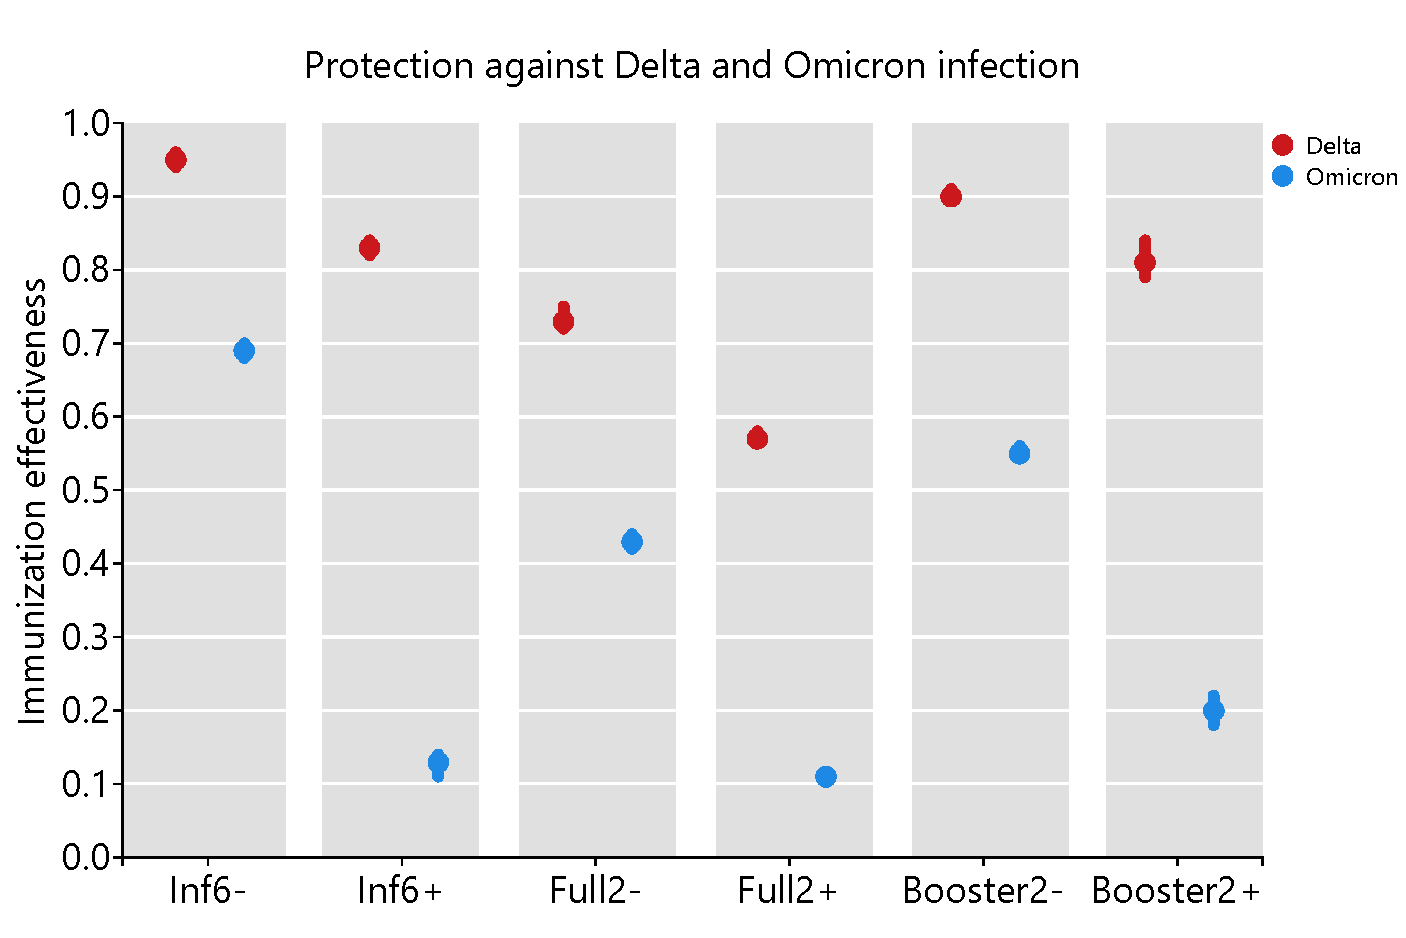
\includegraphics[width=0.9\textwidth]{fig2.pdf}
% \caption{Vaccine-acquired immunity against infection with respect to the delay from the full vaccine application, including the effect of a booster vaccine dose. %adjusted for sex and age.
% }
% \label{resfig2}
% \end{figure}

% A similar trend can be seen in the estimation of vaccine effectiveness against hospital admissions and deaths. For hospital admission, the vaccine effectiveness declined for Comirnaty from 90\% (95\% CI 89-91) at 0-2 months after dose 2 to 75\% (95\% CI 73-76) at 7-8 months, for Spikevax from 94\% (95\% CI 92-96) to 81\% (95\% CI 78-84), and for Vaxzevria from 87\% (95\% CI 81-91) at 0-2 months to 70\% (95\% CI 68-72) at 5-6 months  (Fig.\,\ref{resfig2} red curves, Table \ref{tab:vacc_hazard_ratios}). In the case of protection from death the model estimated for Comirnaty a decrease from 92\% (95\% CI 90-93) at 0-2 months to 83\% (95\% CI 81-86) at 7-8 months, from 96\% (95\% CI 91-98) to 88\% (95\% CI 82-92) for Spikevax within the first 8 months and from 93\% (95\% CI 77-98) to 82\% (95\% CI 78-85) for Vaxzevria within the first 6 months after application (Fig.\,\ref{resfig2} black curves, Table \ref{tab:vacc_hazard_ratios}). Janssen once again exhibits virtually no decline either in the protection against hospitalization starting from 68\% (95\% CI 60-75) at 2 months to 67\% (95\% CI 62-72) at 5-6 months, or deaths starting from 68\% (95\% CI 42-82) and reaching 68\% (95\% CI 53-78) at 5-6 months (Fig.\,\ref{resfig2}, Table \ref{tab:vacc_hazard_ratios}).


\section{Discussion and Conclusions}
\label{sec4}

Our data supports the evidence that the Omicron variant of SARS-CoV-2,  to a significant extent, evades both the post-vaccination and post-infection immunity. The VEs of all the vaccines used in the Czech Republic are lower for Omicron compared to Delta but there is still significant protection by any recent vaccination against severe outcomes. Protection against infection and particularly hospitalization or the need for intensive care is much increased by a recent booster dose; however, as we previously observed with Alpha and Delta \citep{Berec2021preprint}, the protection starts waning after a few weeks. The combined post-infection and post-vaccination immunity is also significantly protective regardless of the exact sequence of events suggesting that the best protective strategy before a coming wave is to vaccinate all individuals, whether previously vaccinated or with a previous covid-19 infection.

%In summary, we used a comprehensive national population-based database containing individual level data about all detected SARS-CoV-2 infection cases to estimate many important characteristics of the post-vaccination and post-infection immunity in the population of the Czech Republic, covering all four vaccines currently approved in the EU and the protection from infection, hospital admission and death. The results strongly advocate for a timely and widespread administration of vaccine booster doses. Covid-19 will undoubtedly continue to disrupt everyday lives and cause suffering and loss of life around the globe and real-life vaccine effectiveness data such as the ones presented in this study can bring an important insight for policy makers in order to limit the worst impacts of the current pandemic.

{\bf Contributors} LB, M\v{S}, and LP conceived this study. JJ, OM, JW, MZ, and TB prepared and checked the data, TP provided the methodological expertise, JW and M\v{S} conducted the analyses. LB and JT wrote the first draft of the manuscript. All authors contributed to writing the manuscript and interpreting the results. All authors approved the final version and had final responsibility for the decision to submit it for publication. 

{\bf Declaration of interests} All other authors declare no competing interests.

{\bf Data sharing} Data reported in this study and used for the analyses is not public. De-identified individual-level data is available to the scientific community. Requests should, together with a short description of their analysis proposals, be submitted to the Institute of Health Information and Statistics of the Czech Republic \\ ({\tt www.uzis.cz/index-en.php}) where they will be assessed based on relevance and scientific merit.

%% The Appendices part is started with the command \appendix;
%% appendix sections are then done as normal sections
%% \appendix

%% \section{}
%% \label{}

%% If you have bibdatabase file and want bibtex to generate the
%% bibitems, please use
%%
\bibliographystyle{elsarticle-harv} 
\bibliography{refs}

%% else use the following coding to input the bibitems directly in the
%% TeX file.

%\begin{thebibliography}{00}

%% \bibitem[Author(year)]{label}
%% Text of bibliographic item

%\bibitem[ ()]{}

%\end{thebibliography}

%%% Supplementary material

\newpage

\section*{Supplementary material}

\setcounter{table}{0}
\renewcommand{\thetable}{S\arabic{table}}
\setcounter{figure}{0}
\renewcommand{\thefigure}{S\arabic{figure}}

%{\bf Data Sharing} \\[1ex]
%The R code for conducting our analyses, together with a sample input data set and complete documentation is (temporarily) available in the following link: \\ \url{github.com/aboubek/index_okresu}

%\newpage
%\vspace{5ex}

\noindent
{\bf Methods: a Cox regression with time-varying covariates}

For both the Omicron and the Delta variant, we use a Cox proportional Hazard model with time varying covariates to asses hazard ratios of various immunity states. In this model,
we brought each individual through several ``immunity states'' {\tt Immunity}. The outcomes (events) are either (a confirmed) infection ({\tt VariantInf}, may be repeated), hospitalization ({\tt VariantHosp}), oxygen therapy ({\tt VariantOxygen}) or ICU admission ({\tt VariantICU}). Undiscriminated infections and infections by the other variant led to withdrawal from the study (right censoring). 
Deaths of covid ({\tt DeadByCov}) or for other reasons ({\tt DeadByOther}) are also recorded, leading to censoring at the time of the event. Fixed (non-time-dependent) covariates include sex ({\tt Sex}) and age category ({\tt AgeGr}). The input for the Cox regression model ({\tt coxph} from {\tt survival} {\tt R} package) consists of one or more records for each subject, each referring to an interval from {\tt T1} to {\tt T2}, containing the values of covariates $Immunity,AgeGr,Sex$ valid in $[T1,T2)$ and indicators of outcomes {\tt VariantInf, VariantHosp, VariantOxygen, VariantICU, DeadByCov, DeadByOther}, happening at $T2$. There may be (and typically are) several records for each subject, each corresponding to a time interval in which the covariates are constant and in the interior of which no events happen.

Time is measured in days and we take the day before our study period (Dec 7th, 2021) as time zero. The {\tt Immunity} categorical covariate can take value {{\tt \_noimmunity}} meaning that the subject was neither vaccinated nor underwent (comfirmed) infection, or it took form {\tt {\em X}\_alone} meaning the condition $X$ happened or the form {\tt {\em X}\_{\em Y}} which means that condition $X$ happened, being followed by condition $Y$ in time. The conditions could be: 
\begin{description}
\item[{\tt part1}] partially vaccinated (from 14 days of the dose application)
\item[{\tt full1}] fully vaccinated no earlier than two months ago (from 14 days to $14+61-1=74$ days after the dose application)
\item[{\tt full2+}] fully vaccinated earlier than two months ago (from 75 days from the application or earlier)
\item[{\tt full1}] booster vaccinated no earlier than two months ago (from 14 days to $74$ days after the dose application)
\item[{\tt full2+}] booster vaccinated earlier than two months ago (from 75 days from the application or earlier)
\item[{\tt inf1}] underwent infection no earlier than six months (180 days) ago 
\item[{\tt inf2+}] underwent infection earlier than six months (180 days) ago. \end{description}

When separately estimating the post-infection immunity we consider infection by a variant as an outcome. As the explanatory variable, we take the delay from the last infection {\tt InfPrior} grouped by four months and the constant covariates {\tt AgeGr} and {\tt Sex}. The {\tt InfPrior} covariate can take the following values 
\begin{description}
\item[{\tt \_noinf}] no previous infection
\item[{\tt inf1}] 60--180 days after the last confirmed infection (the re-infection cannot happen during the first 60 days by definition)
\item[{\tt inf2}] 181--301 days 
\item[{\tt inf3}] 302--422 days 
\item[{\tt inf4+}] any later.
\end{description}


For better understanding, here we show a complete data record of four sample subjects (A0, A1, A2, and A3) determined by the infection analysis. All of them are recorded from T=0 

A0 is not vaccinated and gets infected the last day of the study.
A1 has not been infected before, but gets infected (Day 140) and dies of covid (Day 150) without being vaccinated. A2 became first-dose vaccinated with Comirnaty on day 114, was infected between the first and second dose (day 142), got the second dose (day 220) and survives until the end of the study. A3 has been infected 20 days before beginning of the study, gets vaccinated by Janssen (Day 150) and is not infected through the study's end. 

The input of {\tt coxph} routine is displayed in Table \ref{tab:input}. Note that there is typically more records than events as each follow-up covariate has to have its own interval.

\begin{table}
\caption{Sample input to Cox regression. \vspace{3mm}}
\label{tab:input}
\centering
\begin{tabular}{cccccccclcc}
\hline
Sub- & T1 & T2 & Inf- & Dead- & Dead- & Inf-& Vacc-& Age- & Sex \\
ject & & & ected & Covid & Other & Prior & Status & Gr & \\
\hline
A0 & 0 & 313 & 1 & 0& 0 & \_none & \_unvacc & 40-44 & F\\
A0 & 313 & 314 &0 & 0& 0&1 & \_unvacc & 40-44 & F\\
A1 & 0 & 140 & 1 &0 & 0 &\_none & \_unvacc & 75-79 & F\\
A1 & 140 & 150 & 0 & 1 & 0 & \_none &  \_unvacc & 75-79 & F\\
A2 & 0 & 128(=114+14) & 0& 0 & 0   & \_none &  \_unvacc  & 45-49 & M\\
A2 & 128 & 142 & 1 & 0 & 0 & \_none & P\_first1& 45-49 & M\\
A2 & 142 & 189(=128+61) & 0 & 0 & 0 & 1 & P\_first1& 45-49 & M\\
A2 & 189 & 220 & 0 & 0 &0 & 1 & P\_first2plus& 45-49 & M\\
A2 & 220 & 233(=142+91)  & 0 & 0& 0 & 1 & P1 & 45-49 & M\\
A2 & 233 & 281(=220+61) & 0 & 0 & 0 & 2 & P1 & 45-49 & M\\
A2 & 281 & 314 & 0 & 0 & 0 & 2 & P2 & 45-49 & M\\
A3 & 0 & 71(=0-20+91) & 0 &0 &0 & 1 & \_unvacc & 40-44 & F\\
A3 & 71 & 162(=71+91) & 0 &0 &0 & 2 & \_unvacc & 40-44 & F\\
A3 & 162 & 164(=150+14) & 0 &0 &0 & 3 & \_unvacc & 40-44 & F\\
A3 & 164 & 225(=164+61) & 0 & 0& 0 & 3 & J1 & 40-44 & F\\
%A3 & 225 & 255(=164+91) & 0 & 0& 0 & 3 & J2 & 40-44 & F\\
%A3 & 255 & 286(=225+61) & 0 & 0& 0 & 3 & J2 & 40-44 & F\\
%A3 & 286 & 314  & 0 & 0& 0 & 3 & J3 & 40-44 & F\\
A3 & 225 & 253(=162+91) & 0 & 0& 0 & 3 & J2 & 40-44 & F\\
A3 & 253 & 286(=225+61) & 0 & 0& 0 & rest & J2 & 40-44 & F\\
A3 & 286 & 314  & 0 & 0& 0 & rest & J3 & 40-44 & F\\
\hline
\end{tabular}
\end{table}

\begin{table}
\caption{Details on analyses. $X$DeltaInf -- a dummy equal to one if the VaccStatus value corresponds to vaccine $X$ and the interval $T1 \geq$ Jul-01-2021, $^\star$ -- 61 day periods (otherwise 91 day periods for InfPrior). \vspace{1mm}}
\centering
\begin{tabular}{lccl}
\hline
Analysis & Ages & Event & Covariates \\ \hline
Infections  & all & Infected & 
InfPrior, VaccStatus, Sex, AgeGr \\
Reinfections & all & Infected & InfPrior$^\star$, Sex, AgeGr \\
Hospitalizations & all & Hospitalized & VaccStatus, Sex, AgeGr \\
Deaths & all & DeadByCov & VaccStatus, Sex, AgeGr \\
Boosters & all & Infected &
InfPrior, VaccStatus, Sex, AgeGr \\
Delta March& 70--79 & Infected & InfPrior, VaccStatus, Sex, AgeGr, ADeltaInf,\\
& & & 
\,\,\,\,\,\,\,\, JDeltaInf, MDeltaInf, PDeltaInf \\
Delta April& 55--69 & Infected & dtto. \\
Delta May& 30--54 & Infected & dtto. \\
\hline
\end{tabular}
\end{table}

{\color{blue} The following will be here just in case we use the detailed analysis (not still reedited!)
\begin{description}
\item[{\tt \_Unvacc}:] The subject is not vaccinated (this value is taken as reference).
\item[{\tt \emph{V}\_first1}] The subject is from $14$ to $14+61-1=74$ days after the first dose of vaccine {\tt \emph{V}} but not $14$ days or more after a second dose. {\tt \emph{V}} may be {\tt A}--Vaxzevria, {\tt M}--Spikevax or {\tt P}--Comirnaty.
\item[{\tt \emph{V}\_first2plus}:] The subject is $75$ days or more after the first dose of vaccine {\tt \emph{V}} but not $14$ days or more after a second dose.
\item[{\tt \emph{VX}}:] The subject is between $14+(X-1)*61$ and $14+(X)*61-1$ days after the final dose of vaccine {\tt \emph{V}} but not $7$ days or more after a booster. In addition to {\tt P/M/A}, the vaccine may be also {\tt J} (Janssen).
\item[{\tt \emph{V}boost}:] The subject is $7$ days or more after a booster by vaccine {\tt \emph{V}}.
\end{description}
The {\tt InfPrior} may take the following values:
\begin{description}
\item[{\tt \_None}:] The subject has not been infected previously.
\item[{\tt \emph{X}}:] The subject is from $(X-1)\times p$ to $X\times p - 1$ days after the last positive test for covid, where $p=61$ in the analyses of reinfections an $p=91$ in the remaining analyses.
\item[{\tt rest}:] In reinfection analysis: the subject is $9 \times 61 = 549$ days or more after the last positive test, in the remaining analyses: the subject is $3 \times 91 = 273$ days or more after the last positive test. 
\end{description}
}
By default, for each subject, the intervals cover the entire period from 7 December 2021 to 13 February 2022. The period is shortened if either
\begin{itemize} 
\item The subject is reported to die
\item The subject is reported to obtain booster by Vaxzevria or Janssen
\item The subject is $4 \times 61 + 14 = 258$ days after the final dose and has not yet obtained a booster.
\item The subject is hospitalized (only in the hospitalization analysis)
\item The subject is infected or gets a vaccine (only in the reinfection analysis)
\end{itemize}

\noindent
{\bf Methods: a Logistic regression}

Here, the binary outcomes {\tt Hosp, Oxygen, ICU} corresponding to discriminated infections are explained by dummy {\tt Variant} taking values either {\tt Omicron} or {\tt Delta}, the value of covariate {\tt Immunity} valid at the time of the corresponding infection and constant covariates {\tt AgeGr} anad {\tt Sex}.

\clearpage
\newpage

\noindent
{\bf Supplementary tables}

% \begin{sidewaystable}[h]
\begin{sidewaystable}
[h]
\caption{Descriptive statistics: population and epidemic characteristics in the Czech Republic; ISID = the Czech National Information System of Infectious Diseases. \vspace{2mm}}

% tp get the following tables, run convertool run with command i

\label{description1}
%\begin{small}
\begin{tabular}{c|cc|cc|ccc|cccc}
\hline
 & \multicolumn{4}{c|}{Dataset} & \multicolumn{3}{c|}{Population by 07/12/2021} &
\multicolumn{4}{c}{Events from 07/12/2021} \\ 
Age & Number & Data & \multicolumn{2}{c|}{Dead by 07/12/2021} & From &  Added & Total & Infec- & Hospi- & Dead & Dead \\ 
group &  & errors & covid-19 & other & ISID &   &  & ted & talized & covid-19 & other \\ 
\hline
0-11&434936&23&6&17&434890&932215&1367105&167628&798&1&3\\
12-15&357588&14&0&11&357563&98925&456488&109893&175&1&3\\
16-17&170567&5&2&16&170544&24472&195016&51543&112&0&1\\
18-24&577030&69&6&94&576861&92631&669492&118759&433&0&13\\
25-29&466101&50&21&88&465942&154983&620925&87595&479&1&15\\
30-34&552204&28&48&156&551972&166959&718931&106904&634&5&30\\
35-39&587595&52&76&224&587243&166067&753310&116199&724&13&39\\
40-44&713128&48&151&453&712476&180845&893321&130422&799&19&84\\
45-49&778086&44&298&793&776951&105635&882586&126795&971&38&105\\
50-54&603655&23&455&1109&602068&89015&691083&81047&1029&67&167\\
55-59&581568&23&879&1792&578874&90859&669733&63633&1321&141&251\\
60-64&527736&16&1668&2892&523160&102305&625465&40469&1509&201&427\\
65-69&594362&21&3310&5374&585657&86761&672418&29413&2374&370&727\\
70-74&572325&19&5541&8917&557848&63329&621177&21452&2984&586&1160\\
75-79&418441&15&6670&10490&401266&15935&417201&14150&3165&691&1231\\
80+&445102&9&15014&31314&398765&48761&447526&14703&5983&1640&3304\\
\hline
Total&8380424&459&34145&63740&8282080&2419697&10701777&1280605&23490&3774&7560\\\hline
Errors & No age & 9929 & No sex & 481s \\
\hline
\end{tabular}
%\end{small}
\end{sidewaystable}

\begin{sidewaystable}[h]
%\begin{table}[h]
\caption{Descriptive statistics: vaccine distribution among different age groups until November 20, 2021.  \vspace{2mm}}
\label{description2}
%\begin{small}
\begin{tabular}{c|ccccc|ccccc}
\hline
Age & \multicolumn{5}{c|}{Completed vaccination} & 
\multicolumn{5}{c}{Booster doses} \\
group & Comirnaty & Spikevax & Vaxzevria & Janssen & Total
& Comirnaty & Spikevax & Vaxzevria & Janssen & Total \\ \hline
0-11&38353&55&3&11&38422&175&2&0&0&177\\
12-15&195722&4167&2&2&199893&16844&143&0&0&16987\\
16-17&120102&3052&33&341&123528&18058&689&0&0&18747\\
18-24&394263&26110&2348&44131&466852&105841&13953&2&12&119808\\
25-29&298948&25096&3547&36148&363739&93385&15294&4&10&108693\\
30-34&364532&28912&4877&37250&435571&131736&21530&3&10&153279\\
35-39&395946&31868&7156&37489&472459&165876&25716&10&27&191629\\
40-44&503173&40455&12059&41404&597091&249310&36474&17&33&285834\\
45-49&564756&44639&16643&43925&669963&321021&44898&17&40&365976\\
50-54&440085&37823&17806&34186&529900&274139&39573&19&41&313772\\
55-59&426529&37494&24522&31785&520330&293838&41891&21&40&335790\\
60-64&388409&36335&33399&28237&486380&307892&42194&23&47&350156\\
65-69&426983&45314&60188&27974&560459&381356&54634&39&97&436126\\
70-74&359947&58087&100680&20549&539263&379045&63896&59&128&443128\\
75-79&246125&46985&83302&12442&388854&276509&48422&53&106&325090\\
80+&264910&40559&67123&9655&382247&276295&42481&47&108&318931\\
\hline
Total&5428783&506951&433688&405529&6774951&3291320&491790&314&699&3784123\\
\hline
\end{tabular}
%\end{small}
\end{sidewaystable}

\end{document}

%\endinput
%%
%% End of file `elsarticle-template-harv.tex'.
